\documentclass[tikz,border=6pt]{standalone}
\usepackage{amsmath,amssymb}
\definecolor{inM}{RGB}{31,94,165}\definecolor{inC}{RGB}{214,96,33}
\tikzset{
  m/.style={circle,inner sep=0pt,minimum size=9pt,ball color=inM!85,draw=inM!60!black,line width=0.3pt},
  c/.style={circle,inner sep=0pt,minimum size=9pt,ball color=inC!90,draw=inC!60!black,line width=0.3pt},
  lab/.style={font=\small,fill=white,fill opacity=0.85,text opacity=1,inner sep=1.2pt,rounded corners=1pt},
  e/.style={line width=0.75pt,black!55},
  ec/.style={line width=1.5pt,inC!80!black}}
\begin{document}
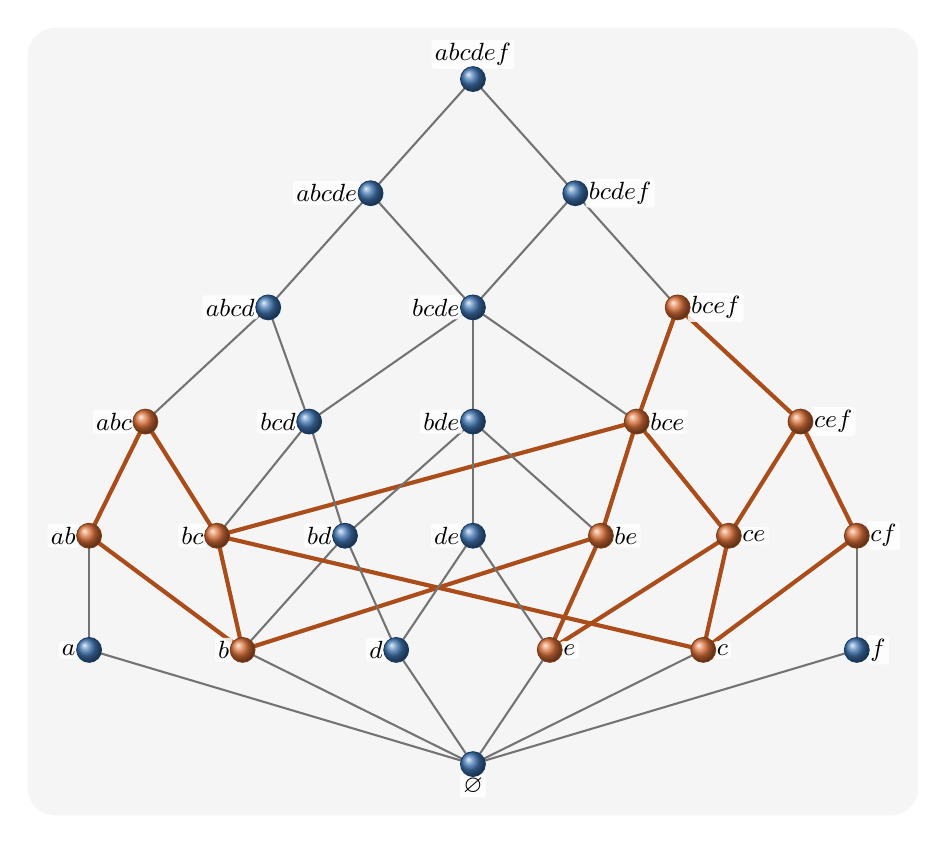
\begin{tikzpicture}[x=1.3cm,y=1.45cm]
\fill[black!4,rounded corners=10pt] (-4.35,-0.45) rectangle (4.35,6.45);
\coordinate (z) at (0.000,0);
\coordinate (a) at (-3.750,1);
\coordinate (b) at (-2.250,1);
\coordinate (c) at (2.250,1);
\coordinate (d) at (-0.750,1);
\coordinate (e) at (0.750,1);
\coordinate (f) at (3.750,1);
\coordinate (ab) at (-3.750,2);
\coordinate (bc) at (-2.500,2);
\coordinate (bd) at (-1.250,2);
\coordinate (be) at (1.250,2);
\coordinate (ce) at (2.500,2);
\coordinate (de) at (0.000,2);
\coordinate (cf) at (3.750,2);
\coordinate (abc) at (-3.200,3);
\coordinate (bcd) at (-1.600,3);
\coordinate (bce) at (1.600,3);
\coordinate (bde) at (0.000,3);
\coordinate (cef) at (3.200,3);
\coordinate (abcd) at (-2.000,4);
\coordinate (bcde) at (0.000,4);
\coordinate (bcef) at (2.000,4);
\coordinate (abcde) at (-1.000,5);
\coordinate (bcdef) at (1.000,5);
\coordinate (X) at (0.000,6);
\draw[e] (z) -- (a);
\draw[e] (z) -- (b);
\draw[e] (z) -- (c);
\draw[e] (z) -- (d);
\draw[e] (z) -- (e);
\draw[e] (z) -- (f);
\draw[e] (a) -- (ab);
\draw[ec] (b) -- (ab);
\draw[ec] (b) -- (bc);
\draw[e] (b) -- (bd);
\draw[ec] (b) -- (be);
\draw[ec] (c) -- (bc);
\draw[ec] (c) -- (ce);
\draw[ec] (c) -- (cf);
\draw[e] (d) -- (bd);
\draw[e] (d) -- (de);
\draw[ec] (e) -- (be);
\draw[ec] (e) -- (ce);
\draw[e] (e) -- (de);
\draw[e] (f) -- (cf);
\draw[ec] (ab) -- (abc);
\draw[ec] (bc) -- (abc);
\draw[e] (bc) -- (bcd);
\draw[ec] (bc) -- (bce);
\draw[e] (bd) -- (bcd);
\draw[e] (bd) -- (bde);
\draw[ec] (be) -- (bce);
\draw[e] (be) -- (bde);
\draw[ec] (ce) -- (bce);
\draw[ec] (ce) -- (cef);
\draw[e] (de) -- (bde);
\draw[ec] (cf) -- (cef);
\draw[e] (abc) -- (abcd);
\draw[e] (bcd) -- (abcd);
\draw[e] (bcd) -- (bcde);
\draw[e] (bce) -- (bcde);
\draw[ec] (bce) -- (bcef);
\draw[e] (bde) -- (bcde);
\draw[ec] (cef) -- (bcef);
\draw[e] (abcd) -- (abcde);
\draw[e] (bcde) -- (abcde);
\draw[e] (bcde) -- (bcdef);
\draw[e] (bcef) -- (bcdef);
\draw[e] (abcde) -- (X);
\draw[e] (bcdef) -- (X);
\node[lab,below=3.5pt] at (z) {$\varnothing$};
\node[lab,left=3.5pt] at (a) {$a$};
\node[lab,left=3.5pt] at (b) {$b$};
\node[lab,right=3.5pt] at (c) {$c$};
\node[lab,left=3.5pt] at (d) {$d$};
\node[lab,right=3.5pt] at (e) {$e$};
\node[lab,right=3.5pt] at (f) {$f$};
\node[lab,left=3.5pt] at (ab) {$ab$};
\node[lab,left=3.5pt] at (bc) {$bc$};
\node[lab,left=3.5pt] at (bd) {$bd$};
\node[lab,right=3.5pt] at (be) {$be$};
\node[lab,right=3.5pt] at (ce) {$ce$};
\node[lab,left=3.5pt] at (de) {$de$};
\node[lab,right=3.5pt] at (cf) {$cf$};
\node[lab,left=3.5pt] at (abc) {$abc$};
\node[lab,left=3.5pt] at (bcd) {$bcd$};
\node[lab,right=3.5pt] at (bce) {$bce$};
\node[lab,left=3.5pt] at (bde) {$bde$};
\node[lab,right=3.5pt] at (cef) {$cef$};
\node[lab,left=3.5pt] at (abcd) {$abcd$};
\node[lab,left=3.5pt] at (bcde) {$bcde$};
\node[lab,right=3.5pt] at (bcef) {$bcef$};
\node[lab,left=3.5pt] at (abcde) {$abcde$};
\node[lab,right=3.5pt] at (bcdef) {$bcdef$};
\node[lab,above=3.5pt] at (X) {$abcdef$};
\node[m] at (z) {};
\node[m] at (a) {};
\node[c] at (b) {};
\node[c] at (c) {};
\node[m] at (d) {};
\node[c] at (e) {};
\node[m] at (f) {};
\node[c] at (ab) {};
\node[c] at (bc) {};
\node[m] at (bd) {};
\node[c] at (be) {};
\node[c] at (ce) {};
\node[m] at (de) {};
\node[c] at (cf) {};
\node[c] at (abc) {};
\node[m] at (bcd) {};
\node[c] at (bce) {};
\node[m] at (bde) {};
\node[c] at (cef) {};
\node[m] at (abcd) {};
\node[m] at (bcde) {};
\node[c] at (bcef) {};
\node[m] at (abcde) {};
\node[m] at (bcdef) {};
\node[m] at (X) {};
\end{tikzpicture}
\end{document}
